%%%%%%%%%%%%%%%%%%%%%%%%%%%%%%%%%%%%%%%%%%%%%%%%%%%%%%%%%%%%%%%%%%%%%%%%%%%%%%%%%%%%%%%%%%%%%%%%
%
% CSCI 1430 Written Question Template
%
% This is a LaTeX document. LaTeX is a markup language for producing documents.
% Your task is to answer the questions by filling out this document, then to
% compile this into a PDF document.
%
% TO COMPILE:
% > pdflatex thisfile.tex

% If you do not have LaTeX, your options are:
% - VSCode extension: https://marketplace.visualstudio.com/items?itemName=James-Yu.latex-workshop
% - Online Tool: https://www.overleaf.com/ - most LaTeX packages are pre-installed here (e.g., \usepackage{}).
% - Personal laptops (all common OS): http://www.latex-project.org/get/ 
%
% If you need help with LaTeX, please come to office hours.
% Or, there is plenty of help online:
% https://en.wikibooks.org/wiki/LaTeX
%
% Good luck!
% Srinath and the 1430 staff
%%%%%%%%%%%%%%%%%%%%%%%%%%%%%%%%%%%%%%%%%%%%%%%%%%%%%%%%%%%%%%%%%%%%%%%%%%%%%%%%%%%%%%%%%%%%%%%%
%
% How to include two graphics on the same line:
%
% \includegraphics[width=0.49\linewidth]{yourgraphic1.png}
% \includegraphics[width=0.49\linewidth]{yourgraphic2.png}
%
% How to include equations:
%
% \begin{equation}
% y = mx+c
% \end{equation}
%
%%%%%%%%%%%%%%%%%%%%%%%%%%%%%%%%%%%%%%%%%%%%%%%%%%%%%%%%%%%%%%%%%%%%%%%%%%%%%%%%%%%%%%%%%%%%%%%%

\documentclass[11pt]{article}

\usepackage[english]{babel}
\usepackage[utf8]{inputenc}
\usepackage{amssymb}
\usepackage{xcolor}
\usepackage[colorlinks = true,
            linkcolor = blue,
            urlcolor  = blue]{hyperref}
\usepackage[a4paper,margin=1.5in]{geometry}
\usepackage{stackengine,graphicx}
\usepackage{fancyhdr}
\setlength{\headheight}{15pt}
\usepackage{microtype}
\usepackage{times}
\usepackage[shortlabels]{enumitem}
\setlist[enumerate]{topsep=0pt}
\usepackage{amsmath}
\usepackage{framed}
\usepackage{mdframed}
\usepackage{xcolor}
\usepackage[most]{tcolorbox}
\usepackage{booktabs}

% a great python code format: https://github.com/olivierverdier/python-latex-highlighting
\usepackage{pythonhighlight}

\usepackage{trimclip,lipsum}

\frenchspacing
\setlength{\parindent}{0cm} % Default is 15pt.
\setlength{\parskip}{0.3cm plus1mm minus1mm}

\pagestyle{fancy}
\fancyhf{}
\lhead{Homework 5 Written Questions}
\rhead{CSCI 1430}
\lfoot{\textcolor{red}{\textbf{Only}
\ifcase\thepage
\or \textbf{instructions}
\or \textbf{A1 (a)}
\or \textbf{A1 (b)}
\or \textbf{A2 (a)}
\or \textbf{A2 (b)}
\or \textbf{A3 (a) - (b)}
\or \textbf{A3 (c)}
\or \textbf{A4 (a) - (c)}
\or \textbf{A4 (d) - (f)}
\or \textbf{A4 (g) - (i)}
\or \textbf{A5}
\or \textbf{Q6}
\or \textbf{Q6}
\or \textbf{Q6}
\or \textbf{A6 (a)}
\or \textbf{A6 (b)}
\or \textbf{discussion attendance}
\or \textbf{feedback}
\else
\textbf{[ERROR: PAGE MISALIGNMENT]}
\fi
\textbf{should be on this page}
}}
\rfoot{\thepage~/ 15}


\date{}

\title{\vspace{-1cm}Homework 5 Written Questions}


\begin{document}
\maketitle
\vspace{-3cm}
\thispagestyle{fancy}

\section*{ Document Instructions}
\begin{itemize}

  \item 6 questions \textbf{[8 + 8 + 6 + 11 + 4 + 8 = 45 + 3 bonus points]}.
  \item Fill all your answers within the answer boxes, and \textbf{please do NOT remove the answer box outlines}.
  \item Questions are highlighted in the \textbf{orange boxes}, bonus questions are highlighted in \textbf{blue boxes}, answers should be recorded in the \textbf{green boxes}.
  \item Include code, images, and equations where appropriate.
  \item To identify all places where your responses are expected, search for `TODO'.
  \item The answer box sizes have been set by the staff beforehand and will truncate your text if it goes beyond the limit. Please make sure your responses fit in the appropriate spaces. \textbf{Extra pages are not permitted unless otherwise specified.}
  \item Make sure your submission has the right number of pages to validate page alignment sanity (check the footer).
  \item Please make this document anonymous.
\end{itemize}

\section*{ Gradescope Instructions}
\begin{itemize}
  \item When you are finished, compile this document to a PDF and submit it directly to Gradescope. 
  \item The pages will be automatically assigned to the right questions on Gradescope \textit{assuming you do not add any unnecessary pages}. \textbf{Inconsistently assigned pages will lead to a deduction of 2 points per misaligned page (capped at a maximum 6 point deduction).}
\end{itemize}

\pagebreak

%%%%%%%%%%%%%%%%%%%%%%%%%%%%%%%%%%%
\paragraph{Q1:} \textbf{[8 points]} Many traditional computer vision algorithms use convolutional filters to extract feature representations, e.g., in SIFT, to which we then often apply machine learning classification techniques. Convolutional neural networks also use filters within a machine learning algorithm.

\begin{enumerate} [(a)]
\item \textbf{[4 points]}

\begin{tcolorbox}[colback=orange!5!white,colframe=orange!75!black]
What is different about the construction of the filters in each of these approaches? \textbf{[3-4 sentences]}
\end{tcolorbox}
\begin{tcolorbox}[colback=white!5!white,colframe=green!75!black]
    \setbox0=\hbox{\parbox[t]{\textwidth}{
    %%%%%%% ANSWER STARTS HERE %%%%%%%%%%%%%%%%%%%%%%%%%%%%
    
    TODO: Your answer for (a) here %%%%%% Remove this line in your answer! %%%%%%
    
    %%%%%%% ANSWER ENDS HERE %%%%%%%%%%%%%%%%%%%%%%%%%%%%%%
    }}
    \clipbox{0pt \dimexpr\dp0-16\baselineskip\relax{} 0in 0pt}{\copy0}
\end{tcolorbox}

\item \textbf{[4 points]}

\begin{tcolorbox}[colback=orange!5!white,colframe=orange!75!black]
Please declare and explain at least two advantages and disadvantages of each of these two approaches. \textbf{[6-7 sentences]}
\end{tcolorbox}
\begin{tcolorbox}[colback=white!5!white,colframe=green!75!black]
    \setbox0=\hbox{\parbox[t]{\textwidth}{
    %%%%%%% ANSWER STARTS HERE %%%%%%%%%%%%%%%%%%%%%%%%%%%%
    
    TODO: Your answer for (b) here %%%%%% Remove this line in your answer! %%%%%%
    
    %%%%%%% ANSWER ENDS HERE %%%%%%%%%%%%%%%%%%%%%%%%%%%%%%
    }}
    \clipbox{0pt \dimexpr\dp0-16\baselineskip\relax{} 0in 0pt}{\copy0}
\end{tcolorbox}
\end{enumerate}

% \paragraph{A1:} Your answer here.
% Uncomment the stencil below and fill in your solution.

% \begin{enumerate}[(a)]

% \item

% \item

% \end{enumerate}


%%%%%%%%%%%%%%%%%%%%%%%%%%%%%%%%%%%
\pagebreak
\paragraph{Q2:} \textbf{[8 points]} Many CNNs have a fully connected multi-layer perceptron (MLP) after the convolutional layers as a general purpose `decision-making' subnetwork. Unlike in convolutional layers and locally connected MLPs, where not every input connects to every perceptron, a fully connected MLP guarantees that every input is conntected to every perceptron.

\begin{tcolorbox}[colback=orange!5!white,colframe=orange!75!black]
What differences in impact could be caused by using a \emph{locally-connected} MLP versus a \emph{fully-connected} MLP, and why?
\end{tcolorbox}

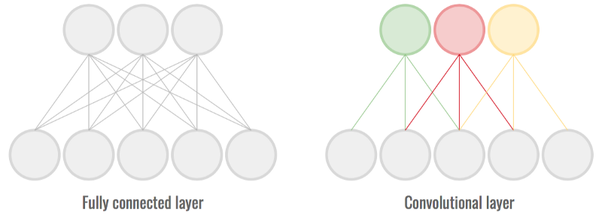
\includegraphics[width=\linewidth]{images/q2mlp.png}

\begin{enumerate} [(a)]
\item \textbf{[4 points]} 
\begin{tcolorbox}[colback=orange!5!white,colframe=orange!75!black]
Explain these differences in terms of learned convolution feature maps, their connections, and the perceptrons in the MLP. \textbf{[5 - 6 sentences]}
\end{tcolorbox}

\begin{tcolorbox}[colback=white!5!white,colframe=green!75!black]
    \setbox0=\hbox{\parbox[t]{\textwidth}{
    %%%%%%% ANSWER STARTS HERE %%%%%%%%%%%%%%%%%%%%%%%%%%%%
    
    TODO: Your answer for (a) here %%%%%% Remove this line in your answer! %%%%%%
    
    %%%%%%% ANSWER ENDS HERE %%%%%%%%%%%%%%%%%%%%%%%%%%%%%%
    }}
    \clipbox{0pt \dimexpr\dp0-16\baselineskip\relax{} 0in 0pt}{\copy0}
\end{tcolorbox}

\pagebreak
\item \textbf{[4 points]}
\begin{tcolorbox}[colback=orange!5!white,colframe=orange!75!black]
Explain these differences in the context of a few different real world examples of computer vision. What cases would a locally connected MLP work better than a fully connected MLP? What could be the stakes if the wrong type of MLP is chosen? \textbf{[5 - 6 sentences]}
\end{tcolorbox}

\begin{tcolorbox}[colback=white!5!white,colframe=green!75!black]
    \setbox0=\hbox{\parbox[t]{\textwidth}{
    %%%%%%% ANSWER STARTS HERE %%%%%%%%%%%%%%%%%%%%%%%%%%%%
    
    TODO: Your answer for (b) here %%%%%% Remove this line in your answer! %%%%%%
    
    %%%%%%% ANSWER ENDS HERE %%%%%%%%%%%%%%%%%%%%%%%%%%%%%%
    }}
    \clipbox{0pt \dimexpr\dp0-16\baselineskip\relax{} 0in 0pt}{\copy0}
\end{tcolorbox}

\end{enumerate}


\pagebreak
\paragraph{Q3:} \textbf{[6 points]} 
\begin{tcolorbox}[colback=orange!5!white,colframe=orange!75!black]
Given a neural network classifier and the stochastic gradient descent training approach, discuss how the following hyperparameters might affect the training process and outcome.
\end{tcolorbox}

\begin{enumerate}[(a)]
    \item \textbf{[2 points]} Learning rate \textbf{[4-6 sentences]}
    \begin{tcolorbox}[colback=white!5!white,colframe=green!75!black]
    \setbox0=\hbox{\parbox[t]{\textwidth}{
    %%%%%%% ANSWER STARTS HERE %%%%%%%%%%%%%%%%%%%%%%%%%%%%
    
    TODO: Your answer for (a) here %%%%%% Remove this line in your answer! %%%%%%
    
    %%%%%%% ANSWER ENDS HERE %%%%%%%%%%%%%%%%%%%%%%%%%%%%%%
    }}
    \clipbox{0pt \dimexpr\dp0-12\baselineskip\relax{} 0in 0pt}{\copy0}
    \end{tcolorbox}
    \item \textbf{[2 points]} Batch size \textbf{[4-6 sentences]}
    \begin{tcolorbox}[colback=white!5!white,colframe=green!75!black]
    \setbox0=\hbox{\parbox[t]{\textwidth}{
    %%%%%%% ANSWER STARTS HERE %%%%%%%%%%%%%%%%%%%%%%%%%%%%
    
    TODO: Your answer for (b) here %%%%%% Remove this line in your answer! %%%%%%
    
    %%%%%%% ANSWER ENDS HERE %%%%%%%%%%%%%%%%%%%%%%%%%%%%%%
    }}
    \clipbox{0pt \dimexpr\dp0-12\baselineskip\relax{} 0in 0pt}{\copy0}
    \end{tcolorbox}
    \item \textbf{[2 points]} Number of epochs  \textbf{[4-6 sentences]}
    \begin{tcolorbox}[colback=white!5!white,colframe=green!75!black]
    \setbox0=\hbox{\parbox[t]{\textwidth}{
    %%%%%%% ANSWER STARTS HERE %%%%%%%%%%%%%%%%%%%%%%%%%%%%
    
    TODO: Your answer for (c) here %%%%%% Remove this line in your answer! %%%%%%
    
    %%%%%%% ANSWER ENDS HERE %%%%%%%%%%%%%%%%%%%%%%%%%%%%%%
    }}
    \clipbox{0pt \dimexpr\dp0-12\baselineskip\relax{} 0in 0pt}{\copy0}
    \end{tcolorbox}
\end{enumerate}

\pagebreak
\paragraph{Q4:} \textbf{[11 + 1 bonus points]} What effects are caused by adding a spatial max pooling layer (stride $>$ 1) after a single convolutional layer, where the output with max pooling is some size larger than $1 \times 1 \times d$?

There may be multiple correct answers per question.

\emph{Note:} `Global' here means whole image; `local' means only in some image region.

\emph{Tip:} To fill in boxes, replace `\textbackslash square' with `\textbackslash blacksquare' for your answer.

% \paragraph{A4:} Multiple choice. Choose all that apply.

%%% See the tex for the bottom of the page to leave the optional written justification %%%

\begin{enumerate}[(a)]
    \item \textbf{[1 point]}
    \begin{tcolorbox}[colback=orange!5!white,colframe=orange!75!black]
    What happens to the computational cost of training?
    \end{tcolorbox}
    \begin{tcolorbox}[colback=white!5!white,colframe=green!75!black]
    TODO: Select the right option %%%%%% Remove this line in your answer! %%%%%%
    
\begin{tabular}[h]{lr}
\toprule
Increases & $\square$ \\
Decreases & $\square$ \\
\bottomrule
\end{tabular}
\end{tcolorbox}
    
    \item \textbf{[1 point]}
    \begin{tcolorbox}[colback=orange!5!white,colframe=orange!75!black]
    What happens to the computational cost of testing?
    \end{tcolorbox}
    \begin{tcolorbox}[colback=white!5!white,colframe=green!75!black]
    TODO: Select the right option %%%%%% Remove this line in your answer! %%%%%%
    
\begin{tabular}[h]{lr}
\toprule
Increases & $\square$ \\
Decreases & $\square$ \\
\bottomrule
\end{tabular}
    \end{tcolorbox}

    \item \textbf{[2 points]} Read \href{https://interestingengineering.com/innovation/training-ai-is-shockingly-costly-to-the-environment}{this article} about the environmental impacts that deep learning can have. 
    \begin{tcolorbox}[colback=orange!5!white,colframe=orange!75!black]
    How does the implementation of this max pooling layer and its resulting implications for the model's computational costs fit into this discussion? \textbf{[3-4 sentences]}
    \end{tcolorbox}

    \begin{tcolorbox}[colback=white!5!white,colframe=green!75!black]
    \setbox0=\hbox{\parbox[t]{\textwidth}{
    %%%%%%% ANSWER STARTS HERE %%%%%%%%%%%%%%%%%%%%%%%%%%%%
    
    TODO: Your answer for (c) here %%%%%% Remove this line in your answer! %%%%%%
    
    %%%%%%% ANSWER ENDS HERE %%%%%%%%%%%%%%%%%%%%%%%%%%%%%%
    }}
    \clipbox{0pt \dimexpr\dp0-10\baselineskip\relax{} 0in 0pt}{\copy0}
    \end{tcolorbox}

    \pagebreak
    \item \textbf{[1 point]}
    \begin{tcolorbox}[colback=orange!5!white,colframe=orange!75!black]
    What happens to overfitting?
    \end{tcolorbox}
    \begin{tcolorbox}[colback=white!5!white,colframe=green!75!black]
    TODO: Select the right option %%%%%% Remove this line in your answer! %%%%%%

\begin{tabular}[h]{lr}
\toprule
Increases & $\square$ \\
Decreases & $\square$ \\
\bottomrule
\end{tabular}
    \end{tcolorbox}

    \item \textbf{[1 point]}
    \begin{tcolorbox}[colback=orange!5!white,colframe=orange!75!black]
    What happens to underfitting?
    \end{tcolorbox}
    \begin{tcolorbox}[colback=white!5!white,colframe=green!75!black]
    TODO: Select the right option %%%%%% Remove this line in your answer! %%%%%%

\begin{tabular}[h]{lr}
\toprule
Increases & $\square$ \\
Decreases & $\square$ \\
\bottomrule
\end{tabular}
    \end{tcolorbox}

    \item \textbf{[2 points]} 
    \begin{tcolorbox}[colback=orange!5!white,colframe=orange!75!black]
    Briefly discuss the tradeoff between overfitting and underfitting in the context of a CNN. Why wouldn't you want to go too far in either direction and what real-world stakeholders might it affect if you do? \textbf{[3 - 5 sentences]}
    \end{tcolorbox}
    \begin{tcolorbox}[colback=white!5!white,colframe=green!75!black]
    \setbox0=\hbox{\parbox[t]{\textwidth}{
    %%%%%%% ANSWER STARTS HERE %%%%%%%%%%%%%%%%%%%%%%%%%%%%
    
    TODO: Your answer for (f) here %%%%%% Remove this line in your answer! %%%%%%
    
    %%%%%%% ANSWER ENDS HERE %%%%%%%%%%%%%%%%%%%%%%%%%%%%%%
    }}
    \clipbox{0pt \dimexpr\dp0-12\baselineskip\relax{} 0in 0pt}{\copy0}
    \end{tcolorbox}
    
    \item \textbf{[1 point]}
    \begin{tcolorbox}[colback=orange!5!white,colframe=orange!75!black]
    What happens to the nonlinearity of the decision function?
    \end{tcolorbox}
    \begin{tcolorbox}[colback=white!5!white,colframe=green!75!black]
    TODO: Select the right option %%%%%% Remove this line in your answer! %%%%%%

\begin{tabular}[h]{lr}
\toprule
Increases & $\square$ \\
Decreases & $\square$ \\
\bottomrule
\end{tabular}
    \end{tcolorbox}

% \pagebreak
\item \textbf{[2 point]}
\begin{tcolorbox}[colback=orange!5!white,colframe=orange!75!black]
Which of the following occur?
\end{tcolorbox}

\begin{tcolorbox}[colback=white!5!white,colframe=green!75!black]
TODO: Select all that apply %%%%%% Remove this line in your answer! %%%%%%

\begin{tabular}[h]{lr}
\toprule
Provides local rotational invariance & $\square$ \\
Provides global rotational invariance & $\square$ \\
Provides local scale invariance & $\square$ \\
Provides global scale invariance & $\square$ \\
Provides local translational invariance & $\square$ \\
Provides global translational invariance & $\square$ \\
\bottomrule
\end{tabular}
\end{tcolorbox}


%%%%%%%%%%%%%%%%%%%%%%%%%%%%%%%%%%%%%
\item
\textbf{(Bonus)} \textbf{[1 point]}
\begin{tcolorbox}[colback=blue!5!white,colframe=blue!75!black]
Given some input to a convolutional layer with stride 2$\times$2 and kernel size 3$\times$3, and ignoring the boundary (not care about pixel values on the edge of the image), what is the minimum number of convolutional filters required to preserve all input information in the output feature map?
\end{tcolorbox}

%%%%%%%%%%%%%%%%%%%%%%%%%%%%%%%%%%%
Multiple choice.

\emph{Tip:} Use command  `\textbackslash bullet' ($\bullet$) to fill in the dots.

\begin{tcolorbox}[colback=white!5!white,colframe=green!75!black]
TODO: Choose one %%%%%% Remove this line in your answer! %%%%%%

\begin{tabular}[h]{lc}
\toprule
0.5 & $\square$ \\
1 & $\square$ \\
2 & $\square$ \\
4 & $\square$ \\
It's impossible & $\square$ \\
\bottomrule
\end{tabular}
\end{tcolorbox}
\end{enumerate}


\pagebreak
\paragraph{Q5:} \textbf{[4 points]} There have been many attempts to interpret CNN predictions:
\begin{itemize}
    \item We saw \href{https://www.cs.cmu.edu/~aharley/vis/conv/}{this website} in class, which visualizes how a CNN predicts numerals when trained on the MNIST dataset.
    
    \item This homework asks you to use \href{https://www.oreilly.com/content/introduction-to-local-interpretable-model-agnostic-explanations-lime/}{LIME} to attempt to explain your model predictions. 

    \item Another option is saliency maps. Please read this \href{https://opendatascience.com/visualizing-your-convolutional-neural-network-predictions-with-saliency-maps/}{short article} describing how saliency maps work, and see more examples \href{https://github.com/jacobgil/pytorch-grad-cam}{here from a saliency map software package}.
\end{itemize}
CNN interpretability remains an open question. For example, in medical imaging, hand designing features from biological experts might lead to a generalizable and explainable method for physicians, regulators, or patients. However, deep learning methods can show \href{https://drive.google.com/file/d/1bDAqEtW482OJeqMBt5A4AradVa4gf_o9/view}{higher test accuracy}, even if their results may be less explainable.

\begin{tcolorbox}[colback=orange!5!white,colframe=orange!75!black]
When is it important to be able to interpret the reasons a machine made a decision, and when is it not? \textbf{[5-7 sentences]}
\end{tcolorbox}

\begin{tcolorbox}[colback=white!5!white,colframe=green!75!black]
\setbox0=\hbox{\parbox[t]{\textwidth}{
%%%%%%% ANSWER STARTS HERE %%%%%%%%%%%%%%%%%%%%%%%%%%%%

TODO: Your answer here %%%%%% Remove this line in your answer! %%%%%%

%%%%%%% ANSWER ENDS HERE %%%%%%%%%%%%%%%%%%%%%%%%%%%%%%
}}
\clipbox{0pt \dimexpr\dp0-16\baselineskip\relax{} 0in 0pt}{\copy0}
\end{tcolorbox}


% Please leave the pagebreak
\pagebreak
%%%%%%%%%%%%%%%%%%%%%%%%%%%%%%%%%%%%%
\paragraph{Q6 background:}
Let us consider using a neural network (non-convolutional) to perform classification on the \href{http://yann.lecun.com/exdb/mnist/}{MNIST dataset} of handwritten digits, with 10 classes covering the digits 0--9. Each image is 28$\times$28 pixels, and so the network input is a 784-dimensional vector $\mathbf{x}=(x_1,x_2,\dots,x_i,\dots,x_{784})$. The output of the neural network is probability distribution $\mathbf{p}=(p_1,\dots,p_j,\dots,p_{10})$ over the 10 classes. Suppose our network has one fully-connected layer with $10$ neurons---one for each class. Each neuron has a weight for each input $\mathbf{w}=(w_1,\dots,w_i,\dots,w_{784})$, plus a bias $b$. As we only have one layer with no multi-layer composition, there's no need to use an activation function.

When we pass in a vector $\mathbf{x}$ to this layer, we will compute a 10-dimensional output vector $\mathbf{l}=(l_1,l_2,...,l_j,...,l_{10})$ as:
\begin{equation}
    l_j = \mathbf{w}_j \cdot \mathbf{x} + b_j = \sum_{i=1}^{784}w_{ij}x_i + b_j
\end{equation}
These distances from the hyperplane are sometimes called `logits' (hence $l$) when they are the output of the last layer of a network. In our case, we only have \emph{one} layer, so our single layer is the last layer.

\hspace{\fill}\rule{0.5\linewidth}{.5pt}\hspace{\fill}

Often we want to talk about the confidence of a classification. So, to turn our logits into a probability distribution $\mathbf{p}$ for our ten classes, we apply the \emph{softmax} function:
\begin{equation}
    p_j = \frac{e^{l_j}}{\sum_je^{l_j}}
   \label{eq:softmax}
\end{equation}
Each $p_j$ will be positive, and $\sum_jp_j = 1$, and so softmax is guaranteed to output a probability distribution. Picking the most probable class provides our network's prediction.

\emph{If} our weights and biases were trained, Eq.~\ref{eq:softmax} would classify a new test example.

\hspace{\fill}\rule{0.5\linewidth}{.5pt}\hspace{\fill}

We have two probability distributions: the true distribution of answers from our training labels $\mathbf{y}$, and the predicted distribution produced by our current classifier $\mathbf{p}$. To train our network, our goal is to define a loss to reduce the distance between these distributions.

Let $y_j=1$ if class $j$ is the true label for $x$, and $y_j = 0$ if $j$ is not the true label. Then, we define the \emph{cross-entropy loss}:
\begin{equation}
    L(w,b,x) = - \sum_{j=1}^{10}y_j\ln(p_j),
\end{equation}
which, after substitution of Eqs. 2 and 1, lets us compute an error (remember that: error = 1 - accuracy) between the labeled ground truth distribution and our predicted distribution.

So...why does this loss $L$ work? Using the cross-entropy loss exploits concepts from information theory---Aur\'{e}lien G\'{e}ron has produced \href{https://www.youtube.com/watch?v=ErfnhcEV1O8}{a video with a succinct explanation of this loss}. Briefly, the loss minimizes the difference in the amounts of information needed to represent the two distributions. Other losses are also applicable, with their own interpretations, but these details are beyond the scope of this course.

%%%%%%%%%%%%%%%%%%%
% Cheat sheet for information theory
%
% Probability distribution \mathbf{p}
% Describes the likelihood of different outcomes, e.g., for our MNIST dataset samples, we might have a 0.09 chance that an image will be of a character '0', 0.11 for a '1', 0.08 for a '2', and so on, with the sum chances for all characters being 1.0.
%
% What is entropy?  H(\mathbf{p}) = - \sum_{i} p_i \log_2{p_i}
% Probability of an event multiplied by the reduction in uncertainty (or amount of information) received from that event. Is the average amount of information (in bits) that you receive from one sample drawn from a probability distribution. It tells you how predictable that probability distribution is (or, written another way, how uncertain we are). 0 entropy = no uncertainty. High entropy = very uncertain probability distribution.
%
% What is cross-entropy?   H(\mathbf{p},\mathbf{q}) = - \sum_{i} p_i \log_2{q_i}
% The average message length in bits _across_ two distributions - the true distribution \mathbf{p} and some predicted distribution \mathbf{q}. If the predicted distribution is equal to the true distribution, then cross-entropy _is_ entropy.
%
% So then what is entropy minus cross-entropy?
% This tells us how different the predicted distribution is from the true distribution. This is called the Kullback-Leibler divergence (or KL-divergence). It is a divergence and not a distance because it doesn't have a `sidedness'.
% D_{KL}(\mathbf{p} || \mathbf{q}) = H(\mathbf{p},\mathbf{q}) - H(\mathbf{p})
%
% Why is it \emph{minus}?   The uncertainty reduction factor from a message is equal to 1 / p(event). So, we would normally compute ln( 1/p(event) ). But ln(1/x) = -ln(x), so we equivalently compute -ln( p(event) ).
%
%%%%%%%%%%%%%%%%%%%

\hspace{\fill}\rule{0.5\linewidth}{.5pt}\hspace{\fill}

Onto the training algorithm. The loss is computed once for every different training example. When every training example has been presented to the training process, we call this an \emph{epoch}. Typically we will train for many epochs until our loss over all training examples is minimized.

Neural networks are usually optimized using gradient descent. For each training example in each epoch, we compute gradients via backpropagation (an application of the chain rule in differentiation) to update the classifier parameters via a learning rate $\lambda$:
\begin{equation}
w_{ij} = w_{ij} - \lambda\frac{\partial L}{\partial w_{ij}}, \\
\end{equation}
\begin{equation}
b_j = b_j - \lambda\frac{\partial L}{\partial b_j}.
\end{equation}

We must deduce $\frac{\partial L}{\partial w_{ij}}$ and $\frac{\partial L}{\partial b_j}$ as expressions in terms of $x_i$ and $p_j$.

\emph{Intuition:} Let's just consider the weights. Recall that our network has one layer of neurons followed by a softmax function. To compute the change in the cross-entropy loss with respect to neuron weights $\frac{\partial L}{\partial w_{ij}}$, we will need to compute and chain together three different terms:
\begin{enumerate}
\itemsep0em
\listparindent0em
\topsep0em
\parsep0em
\partopsep0em
\item The change in the loss with respect to the softmax output $\frac{\delta L}{\delta p_j}$,
\item The change in the softmax output with respect to the neuron output $\frac{\delta p_j}{\delta l_j}$, and
\item The change in the neuron output with respect to the neuron weights $\frac{\delta l_j}{w_{ij}}$.
\end{enumerate}
We must derive each individually, and then formulate the final term via the chain rule. The biases follow in a similar fashion.

The derivation is beyond the scope of this class, and so we provide them here:
\begin{equation}
\frac{\delta L}{\delta w_{ij}} = \frac{\delta L}{\delta p_a} \frac{\delta p_a}{\delta l_j} \frac{\delta l_j}{w_{ij}} =\begin{cases}
x_i(p_j-1), a = j\\
x_ip_j,  a\neq j
\end{cases}
\label{eq:wupdate}
\end{equation}
\begin{equation}
\frac{\delta L}{\delta b_j} = \frac{\delta L}{\delta p_a} \frac{\delta p_a}{\delta l_j} \frac{\delta l_j}{b_j} =\begin{cases}
(p_j-1), a = j\\
p_j,  a\neq j
\end{cases}
\label{eq:bupdate}
\end{equation}
Here, $a$ is the predicted class label and $j$ is the true class label. An alternative form you might see shows $\frac{\delta L}{\delta w_{ij}} = x_i(p_j-y_j)$ and $\frac{\delta L}{\delta b_j} = p_j-y_j$ where $y_j=1$ if class $j$ is the true label for $x$, and $y_j = 0$ if $j$ is not the true label.

So...after all of that, our gradient update rules are surprisingly simple!

\emph{Further details:} For interested students, we refer students to Chapter 1 of \href{https://cs.brown.edu/courses/csci1460/assets/files/deep-learning.pdf}{Prof.~Charniak's deep learning notes}, which derives these gradient update rules. We also refer to \href{https://www.ics.uci.edu/~pjsadows/notes.pdf}{Prof.~Sadowski's notes on backpropagation}: Section 1 derives terms first for cross-entropy loss with logistic (sigmoid) activation, and then Section 2 derives terms for cross-entropy loss with softmax. The Wikipedia article on \href{https://en.wikipedia.org/wiki/Backpropagation}{the backpropagation algorithm} likewise represents a derivation walkthrough of the general case with many hidden layers each with sigmoid activation functions, and a final layer with a softmax function.

\hspace{\fill}\rule{0.5\linewidth}{.5pt}\hspace{\fill}


\paragraph{Q6:} We will implement these steps in code using numpy. We provide a code stencil \texttt{main.py} which loads one of two datasets: MNIST and the scene recognition dataset from Homework 4. We also provide two models: a neural network, and then a neural network whose logits are used as input to an SVM classifier. Please look at the comments in \texttt{main.py} for the arguments to pass in to the program for each condition. The neural network model is defined in \texttt{model.py}, and the parts we must implement are marked with TODO comments.

\begin{tcolorbox}[colback=orange!5!white,colframe=orange!75!black]
\emph{Tasks:} Please follow the steps to implement the forward model evaluation and backward gradient update steps. Then, run your model on all four conditions and report training loss (calculated using \emph{training} set) and accuracy (calculated using \emph{testing} set) as the number of training epochs increases.
\\
\\
Please upload your completed \texttt{model.py} to Gradescope under the assignment titled "Homework 5 Written (Numpy)". The autograder will check that you correctly implemented parts of your model. Then, complete the following questions.
\end{tcolorbox}
\pagebreak
\begin{enumerate} [(a)]
    \item \textbf{[4 points]}
    \begin{tcolorbox}[colback=orange!5!white,colframe=orange!75!black]
    How well did each model perform on each dataset?
    \end{tcolorbox}
    \begin{tcolorbox}[colback=white!5!white,colframe=green!75!black]
    %%%%%%%%%%%%%%%%%%%
    %%%%%%%%%%%%%%%%%%%
    % ANSWER STARTS HERE
    % Replace all the 'xx's with your results
        \begin{itemize}
            \item NN on MNIST: xx\% (highest accuracy)
            	\begin{itemize}
            	\item Epoch 0 loss: xx     Accuracy: xx\%
            	\item Epoch 9 loss: xx     Accuracy: xx\%
            	\end{itemize}
            \item NN+SVM on MNIST: xx\% (highest accuracy)
            	\begin{itemize}
            	\item Epoch 0 loss: xx     Accuracy: xx\%
            	\item Epoch 9 loss: xx     Accuracy: xx\%
            	\end{itemize}
            \item NN on SceneRec: xx\% (highest accuracy)
            	\begin{itemize}
            	\item Epoch 0 loss: xx     Accuracy: xx\%
            	\item Epoch 9 loss: xx     Accuracy: xx\%
            	\end{itemize}
            \item NN+SVM on SceneRec: xx\% (highest accuracy)
            	\begin{itemize}
            	\item Epoch 0 loss: xx     Accuracy: xx\%
            	\item Epoch 9 loss: xx     Accuracy: xx\%
        	    s\end{itemize}
        \end{itemize}
    % ANSWER ENDS HERE
    %%%%%%%%%%%%%%%%%%%
    %%%%%%%%%%%%%%%%%%%
    \end{tcolorbox}
    \item \textbf{[4 points]}
    \begin{tcolorbox}[colback=orange!5!white,colframe=orange!75!black]
    What do the training loss and accuracy numbers tell us about a) the capability of the network, b) the complexity of the two problems, and c) the usefulness of the two different classification approaches?
    \end{tcolorbox}
    \begin{tcolorbox}[colback=white!5!white,colframe=green!75!black]
    \setbox0=\hbox{\parbox[t]{\textwidth}{
    %%%%%%% ANSWER STARTS HERE %%%%%%%%%%%%%%%%%%%%%%%%%%%%
    
    TODO: Your answer for (b) here %%%%%% Remove this line in your answer! %%%%%%
    
    %%%%%%% ANSWER ENDS HERE %%%%%%%%%%%%%%%%%%%%%%%%%%%%%%
    }}
    \clipbox{0pt \dimexpr\dp0-18\baselineskip\relax{} 0in 0pt}{\copy0}
    \end{tcolorbox}
    
\end{enumerate}
%%%%%%%%%%%%%%%%%%%%%%%%%%%%%%%%%%%
\pagebreak
\section*{Discussion Attendance:}
\paragraph{Extra Credit:} \textbf{[2 points]}

Please mark this box only if you've attended the discussion session in person.

\begin{tabular}[h]{ll}
$\square$ & I attended the discussion session on DATE \\
\end{tabular}

%%%%%%%%%%%%%%%%%%%%%%%%%%%%%%%%%%%
\pagebreak
\section*{Feedback? (Optional)}
Please help us make the course better. If you have any feedback for this assignment, we'd love to hear it!


% \pagebreak
% \section*{Any additional pages would go here.}


\end{document}
